\def\homeworknumber{5}
\def\homeworkdate{29-11-2011}

\def\umax{u_{\text{max}}}
\def\vmax{v_{\text{max}}}


\documentclass[11pt]{article}
\linespread{1}

\renewcommand{\thefootnote}{\fnsymbol{footnote}}

\usepackage{geometry} % see geometry.pdf on how to lay out the page. There's lots.
\usepackage[utf8]{inputenc}
\usepackage{array}
\usepackage{amsmath,amssymb,latexsym,epic,eepic,epsfig,graphics,psfrag}
\usepackage{amsfonts}
\usepackage{graphicx,float}

\usepackage[danish]{babel}

\usepackage[bottom]{footmisc}

\usepackage{fancyhdr}
\pagestyle{fancy}
\lhead{\small\textit{01246 Partial Differential Equations - Fall 2011 - Anders Hørsted (s082382)}}
\rhead{\thepage}
\chead{}
\lfoot{}\cfoot{}\rfoot{}

\usepackage{pstricks}
\usepackage{pst-node}
\usepackage{wrapfig}
\usepackage{caption}
\usepackage{multirow}
%\usepackage{fouriernc}
%\usepackage[charter]{mathdesign}
\usepackage{lmodern}
\usepackage[normalem]{ulem}
\geometry{a4paper} % or letter or a5paper or ... etc
% \geometry{landscape} % rotated page geometry

\usepackage{subfigure}
\usepackage{placeins}
\usepackage{url}
\usepackage{natbib}
\renewcommand\bibsection*{}
\bibliographystyle{plain}

\makeatletter
\renewcommand*\env@matrix[1][*\c@MaxMatrixCols c]{%
  \hskip -\arraycolsep
  \let\@ifnextchar\new@ifnextchar
  \array{#1}}
\makeatother

\newcommand\myimp{\quad\Leftrightarrow\quad}
\newcommand\half{\frac{1}{2}}
%\newcommand\myvec[1]{\mathbf{#1}}
\newcommand\myvec[1]{\boldsymbol{#1}}
\newcommand\vecx{\myvec{x}}
\newcommand\mymod[1]{\ (\text{mod }#1)}
\newcommand\myreal{\mathbb{R}}
\newcommand\mynatural{\mathbb{N}}
\newcommand\myinteger{\mathbb{Z}}
\newcommand\mycomplex{\mathbb{C}}
\newcommand\myint{\text{int}}
\newcommand\norm[1]{||\,#1\,||}
\newcommand\bignorm[1]{\big|\big|\,#1\,\big|\big|}
\newcommand\seq[1]{\big\{#1\big\}}
\newcommand\smallseq[1]{\{#1\}}
\newcommand\smallseqtoinf[1]{\smallseq{#1}_{k=1}^\infty}
\newcommand\lonew{\ell^1_w}
\newcommand\lone{\ell^1}
\newcommand\ltwo{\ell^2(\mynatural)}
\newcommand\ip[2]{\langle#1,#2\rangle}
\newcommand\hilbert[1]{\mathcal{#1}}
\newcommand\uinf{u_{\infty}}
\newcommand\erf{\text{erf\,}}
\newcommand\infint{\int_{\infty}^{\infty}}
\newcommand\celsius{$^\circ$C}
\newcommand\comsol{Comsol}
\newcommand\fourier{\mathcal{F}}

\usepackage{tabulary}
\newcolumntype{y}{>{\centering\arraybackslash}R}

\setlength{\unitlength}{2mm}
\usepackage{tikz}

\title{Homework \homeworknumber}
\author{01246 Partial differential equations -- \homeworkdate -- Anders Hørsted (s082382)}
%\author{}
\date{} % delete this line to display the current date


\begin{document}
    \maketitle

    \section*{Exercise 1}
    
    An initial value problem for the heat equation with convection is given by
    \begin{gather}\label{eq:pde-ex1}
        u_t - cu_x - du_{xx} = 0, \quad x\in\myreal, t>0 \\
        u(x,0) = g(x),\quad x\in\myreal
    \end{gather}
    where $c,d>0$.

    \subsection*{a)}
    A formula for the solution $u$ is found using the Fourier transform with respect to the $x$ variable. We assume that $u$ has a Fourier transform as a distribution in $x$ and write the Fourier transform as $\hat{u}(k,t)$. The PDE in (\ref{eq:pde-ex1}) can then be written as
    \begin{align*}
        \frac{\text{d}\hat{u}}{\text{d}t} - cik\hat{u} + dk^2\hat{u} &= 0 \myimp\\
        \frac{\text{d}\hat{u}}{\text{d}t} &= (cik - dk^2)\hat{u}
    \end{align*}
    with the initial condition
    \begin{equation}\label{eq:initial-ex1}
        \hat{u}(k, 0) = \hat{g}(k)
    \end{equation}
    For each $k$ this is an first order ODE in $t$ with the general solution
    \begin{equation*}
        \hat{u}(k,t) = A(k)e^{(cik - dk^2)t}
    \end{equation*}
    where $A(k)$ is a constant that may depend on $k$. Using the initial condition (\ref{eq:initial-ex1}) we get the solution
    \begin{equation*}
        \hat{u}(k,t) = \hat{g}(k)e^{(cik - dk^2)t}
    \end{equation*}
    Finally, to get the solution to the PDE the ODE solution $\hat{u}$ is inverse transformed to give
    \begin{align*}
        u(x, t) &= \frac{1}{2\pi}\int_{-\infty}^\infty \hat{g}(k)e^{(cik - dk^2)t}e^{ikx}\,dk\\
            &= \frac{1}{2\pi}\int_{-\infty}^\infty \hat{g}(k)e^{-dtk^2+(ct+x)ik}\,dk
    \end{align*}

    \subsection*{b)}
    We now set $g(x)=e^{-x^2}$. Combining $\fourier(e^{-x^2/2})(k)=\sqrt{2\pi}e^{-k^2/2}$ and $\fourier(f(ax))(k)=\frac{1}{|a|}\fourier(f)\left(\frac{k}{a}\right)$, with $a=\sqrt{2}$, gives
    \begin{equation*}
        \hat{g}(k) = \fourier(e^{-x^2})(k) = \sqrt{\pi}e^{-k^2/4}
    \end{equation*}
    and therefore
    \begin{align*}
        u(x, t) &= \frac{\sqrt{\pi}}{2\pi}\int_{-\infty}^\infty e^{-k^2/4}e^{-dtk^2+(ct+x)ik}\,dk \\
                &= \frac{1}{2\sqrt{\pi}}\int_{-\infty}^\infty e^{-(dt+1/4)k^2+(ct+x)ik}\,dk \\
                &= \frac{1}{\sqrt{4dt+1}}\,e^{-(cx+t)^2/(4dt+1)}
    \end{align*}
    Setting $c=1$ and $d=1/2$, $u$ is now plotted for $t=0,1,\dots,5$ and shown in figure~\ref{fig:ex1-plots-c1}. Also, to test the effect of the convection parameter $c$, the solution $u$ is plotted for $c=0.5,2$ at times $t=0,1,2$ and shown in figure~\ref{fig:ex1-plots-c2}
    \begin{figure}[!ht]
    \centering
    \mbox{\subfigure{\includegraphics[width=55mm]{media/ex1-t0.pdf}} \quad 
            \subfigure{\includegraphics[width=55mm]{media/ex1-t1.pdf}}}
    \mbox{\subfigure{\includegraphics[width=55mm]{media/ex1-t2.pdf}} \quad 
            \subfigure{\includegraphics[width=55mm]{media/ex1-t3.pdf}}}
    \mbox{\subfigure{\includegraphics[width=55mm]{media/ex1-t4.pdf}} \quad 
            \subfigure{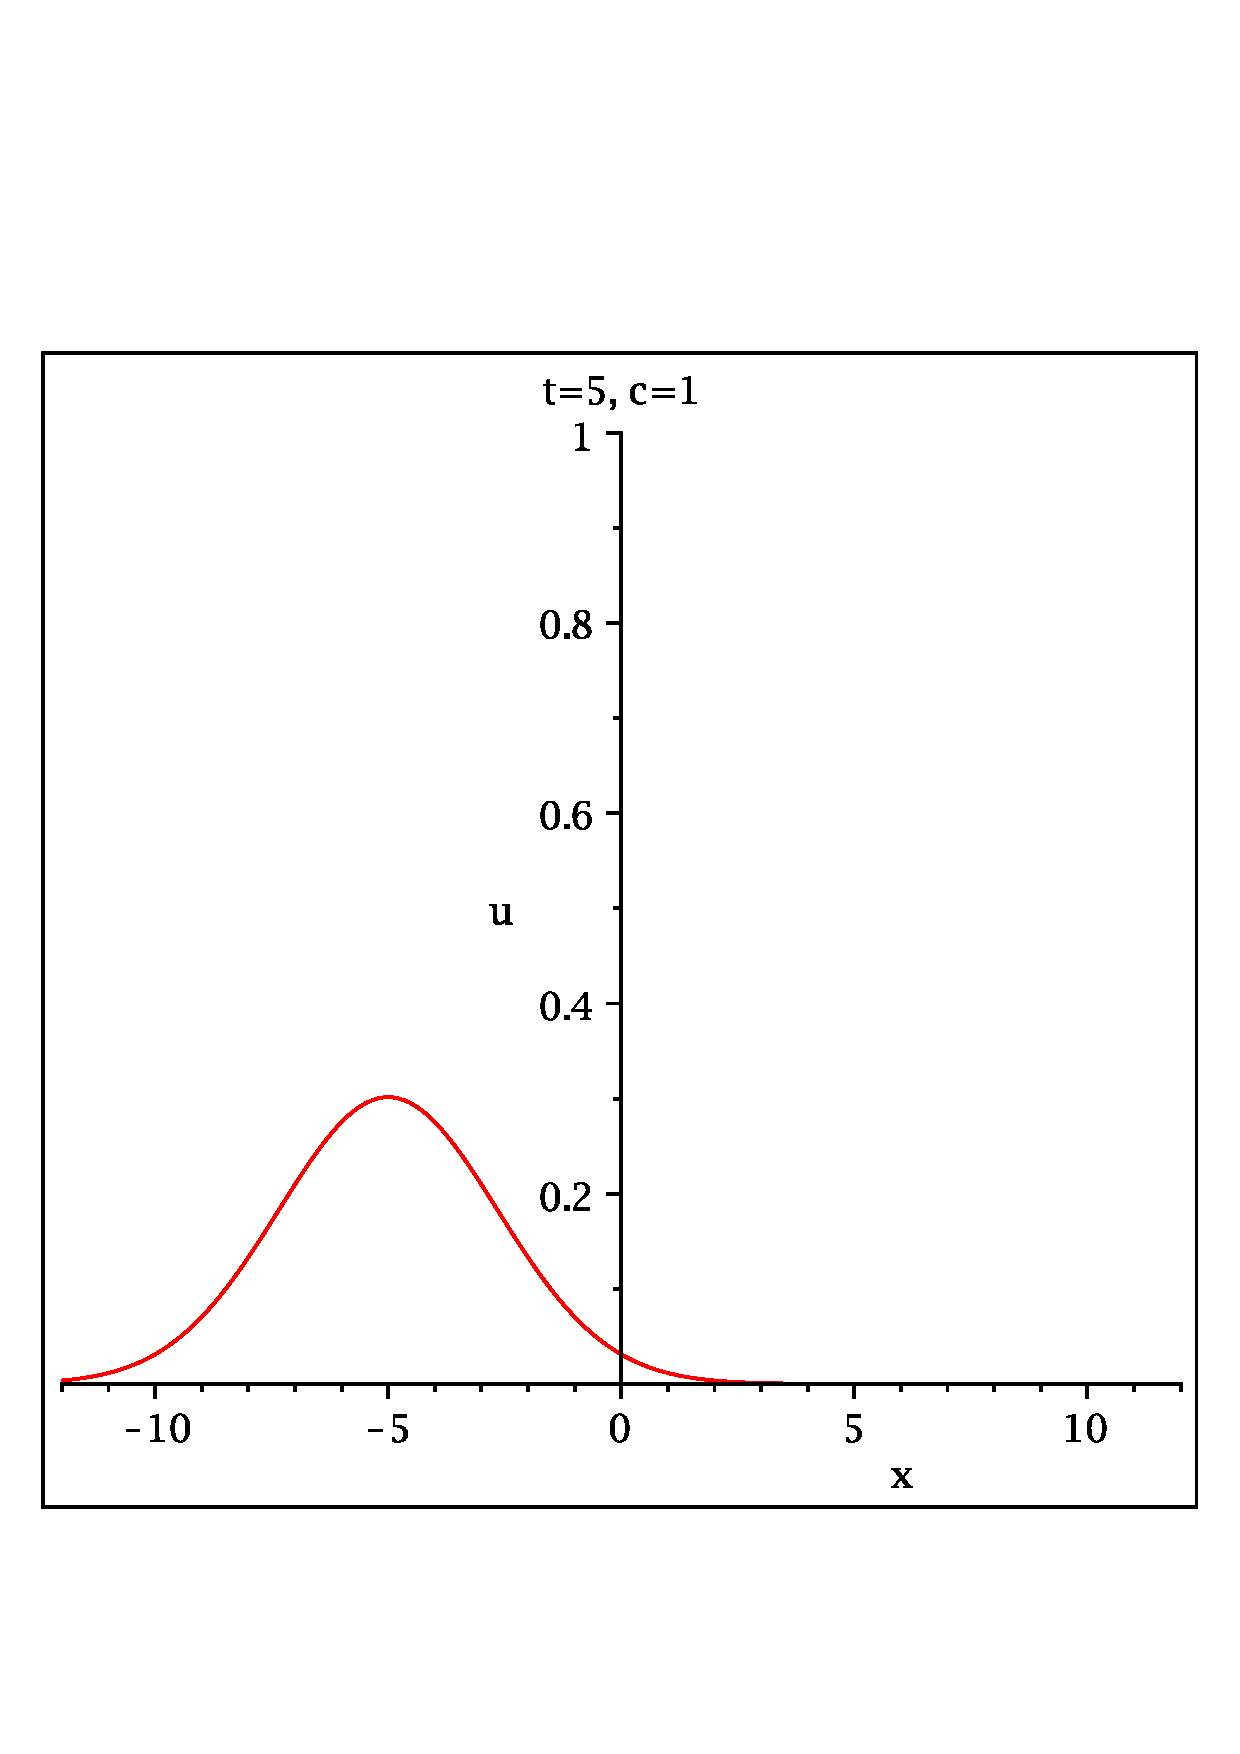
\includegraphics[width=55mm]{media/ex1-t5.pdf}}}
    \caption{Plots of the solution $u$ of exercise 1, for $c=1$ and at times $t=0,1\dots,5$}
    \label{fig:ex1-plots-c1}
    \end{figure}

    \begin{figure}[!ht]
    \centering
    \mbox{\subfigure{\includegraphics[width=55mm]{media/ex1-t0-c05.pdf}} \quad 
            \subfigure{\includegraphics[width=55mm]{media/ex1-t0-c2.pdf}}}
    \mbox{\subfigure{\includegraphics[width=55mm]{media/ex1-t1-c05.pdf}} \quad 
            \subfigure{\includegraphics[width=55mm]{media/ex1-t1-c2.pdf}}}
    \mbox{\subfigure{\includegraphics[width=55mm]{media/ex1-t2-c05.pdf}} \quad 
            \subfigure{\includegraphics[width=55mm]{media/ex1-t2-c2.pdf}}}
    \caption{Plots of the solution $u$ of exercise 1 for different $c$ values. In the left column $c=0.5$ and in the right $c=2$.}
    \label{fig:ex1-plots-c2}
    \end{figure}

    \subsection*{c)}
    
    From figure~\ref{fig:ex1-plots-c1} it is seen that the addition of the convection term in the PDE, adds an macroscopic motion to the heat. This is seen from the maximum density that moves left as time increases. The movement is expected since heat convection is more or less defined as the bulk (or visible) movement of heat. From figure~\ref{fig:ex1-plots-c1} it is also noticed that the diffusion seems unaffected by the convection.

    In figure~\ref{fig:ex1-plots-c2} the solution $u$ is plotted for different values of $c$. Looking at the plots it looks as if $c$ can be interpreted as the speed of the convective movement.

    \FloatBarrier

    \section*{Exercise 2}

    A flow of cars is modelled by
    \begin{gather}\label{eq:pde-ex2}
        u_t + \vmax\left(1-\frac{2u}{\umax}\right)u_x = 0
    \end{gather}
    where $u(x,t)$ is the density of cars at point $x\in\myreal$ at time $t>0$. $\vmax$ is the maximal speed of cars and $\umax$ is the maximal density. In this exercise we set $\vmax=35$ and $\umax=45$. We can model a traffic light at $x=0$, that turns green at time $t=0$, as the initial condition
    \begin{equation}\label{eq:initial-ex2}
        u(x,0) = \phi_1(x) = \begin{cases}
            \umax, & x < 0 \\
            0, & x>0
        \end{cases}
    \end{equation}

    \subsection*{a)}
    We now draw some characteristic curves for the problem. Using the notation of the textbook we have
    \begin{equation*}
        a(u) = \vmax\left(1 - \frac{2u}{\umax}\right)
    \end{equation*}
    and, as mentioned on the bottom of page 384 in the textbook, all characteristic curves are straight lines. Now, for any point $(x,0)$ where $x>0$ we have a characteristic curve through that point with slope
    \begin{equation*}
        \frac{1}{a(\phi_1(x))} = \frac{1}{a(0)} = \frac{1}{\vmax}
    \end{equation*}
    and likewise, for any point $(x,0)$ where $x<0$ the slope of the characteristic curve through that point is 
    \begin{equation*}
        \frac{1}{a(\phi_1(x))} = \frac{1}{a(\umax)} = -\frac{1}{\vmax}
    \end{equation*}
    The characteristic curves with slope of $\pm\frac{1}{\vmax}$ covers all points in the $xt$-plane where $x\leq-t\vmax\lor x\geq t\vmax$, and for all characteristic curves through points where $x\in(-t\vmax,t\vmax)$ we may assume that the characteristic curves passes through origo. Some of the characteristic curves can therefore be plotted and are shown in figure~\ref{fig:chars-q2}

    \begin{figure}[!ht]
        \centering
        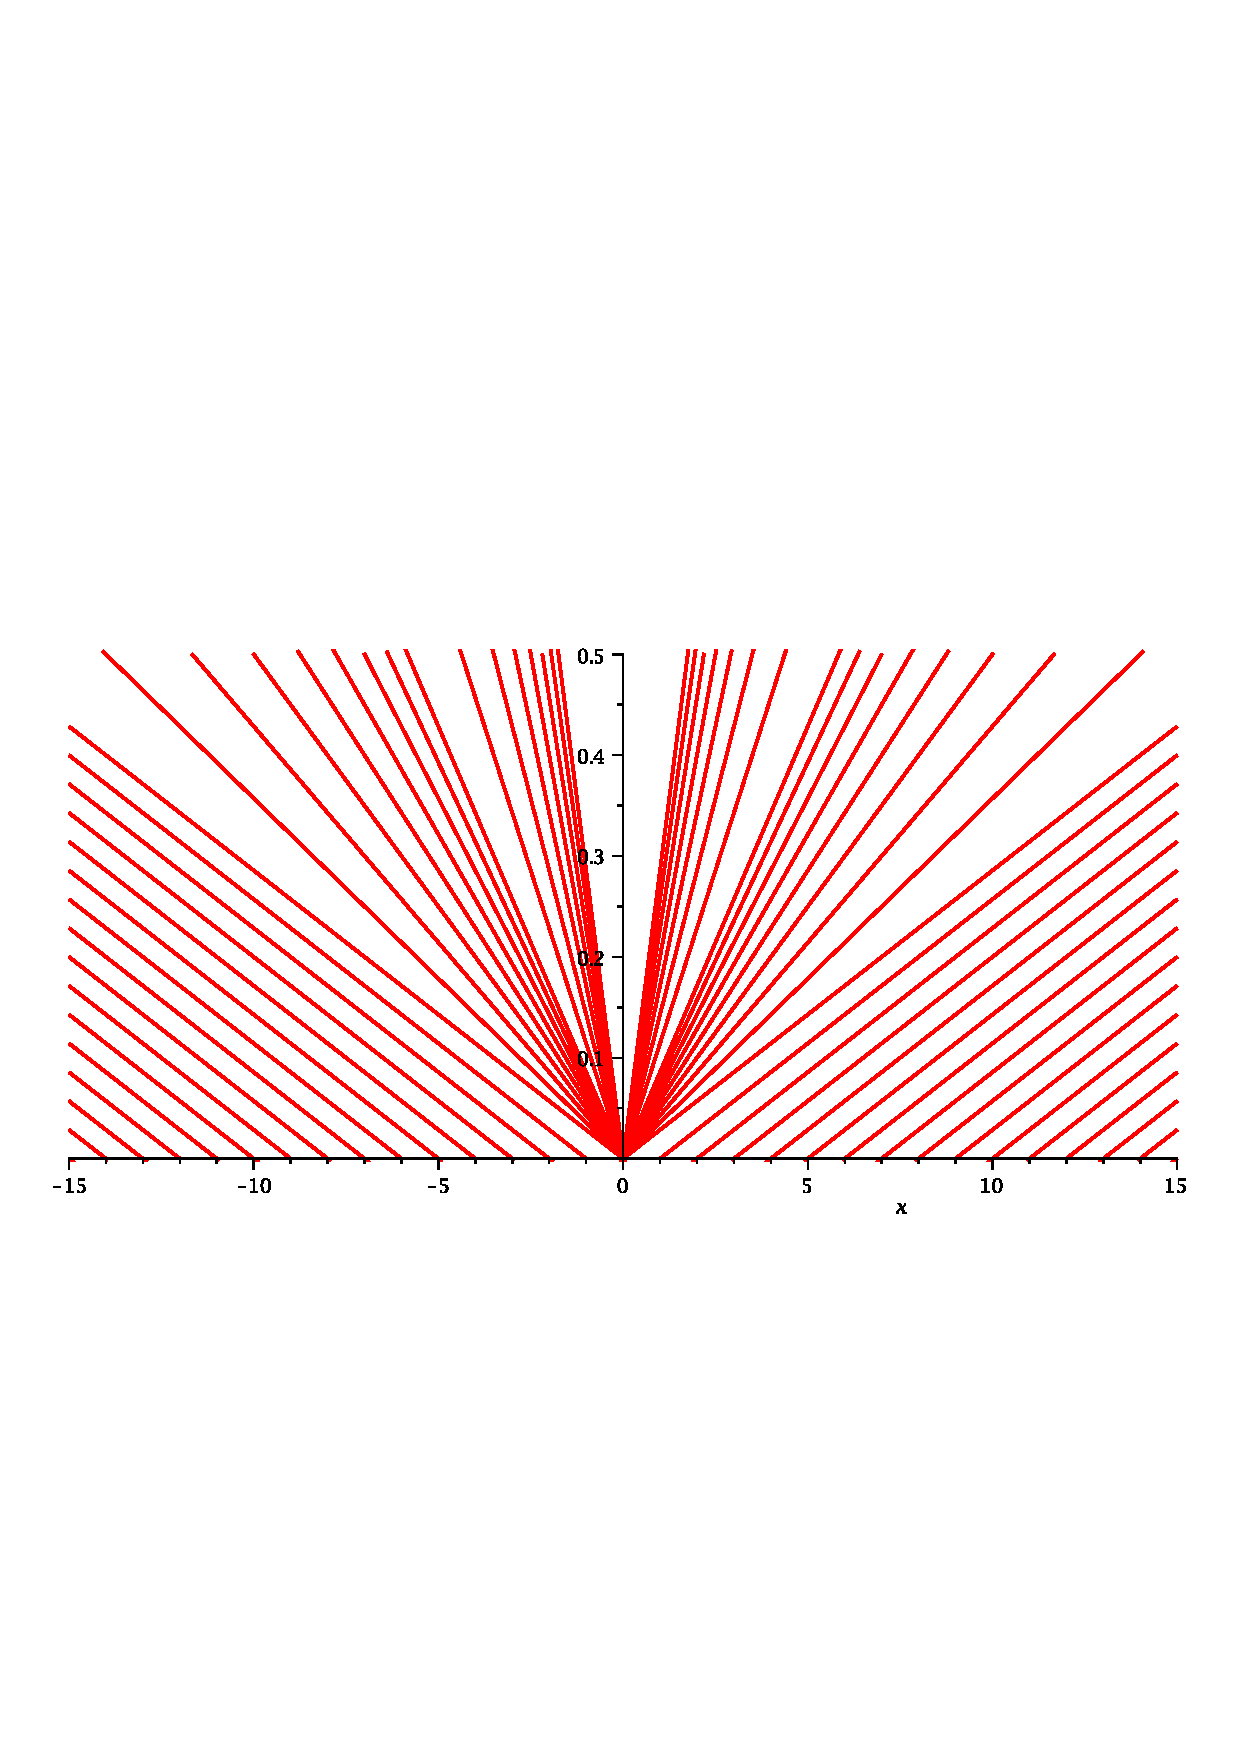
\includegraphics[width=100mm]{media/characteristics-ex2.pdf}
        \caption{Characteristic curves for exercise 2.a}
        \label{fig:chars-q2}
    \end{figure}

    \subsection*{b)}
    The PDE (\ref{eq:pde-ex2}) with the initial condition in (\ref{eq:initial-ex2}) is now solved. In the previous exercise we saw that any point $(x,t)$ where $x>t\vmax$ have a characteristic curve that crosses the $x$-axis on the positive side. Likewise any point where $x<-t\vmax$ have a characteristic curve that crosses the $x$-axis on the negative side. Using the initial condition and the fact that the solution is constant on a charactestic curve (textbook bottom p. 384), gives
    \begin{equation*}
        u(x,t) = \begin{cases}
            \umax & x < -t\vmax \\
            0 & x>t\vmax
        \end{cases}
    \end{equation*}
    For any point where $-t\vmax<x<t\vmax$ we assume that the characteristic curve passes through origo. From the ``slope'' formula at the top of page 385 in the textbook we get
    \begin{align*}
        \frac{x}{t} &= a(u(x,t)) \\
            &= \vmax\left(1 - \frac{2u(x,t)}{\umax}\right) \myimp \\
        u(x,t) &= \frac{\umax}{2} - \frac{\umax}{2\vmax}\frac{x}{t}
    \end{align*}
    The final solution is therefore given as
    \begin{equation*}
        u(x,t) = \begin{cases}
            \umax & x < -t\vmax \\
            \frac{\umax}{2} - \frac{\umax}{2\vmax}\frac{x}{t} & -t\vmax<x<t\vmax \\
            0 & x>t\vmax
        \end{cases}
    \end{equation*}

    \begin{figure}[!ht]
        \centering
        \mbox{\subfigure{\includegraphics[width=55mm]{media/ex2-t0.pdf}} \quad 
                \subfigure{\includegraphics[width=55mm]{media/ex2-t1.pdf}}}
        \mbox{\subfigure{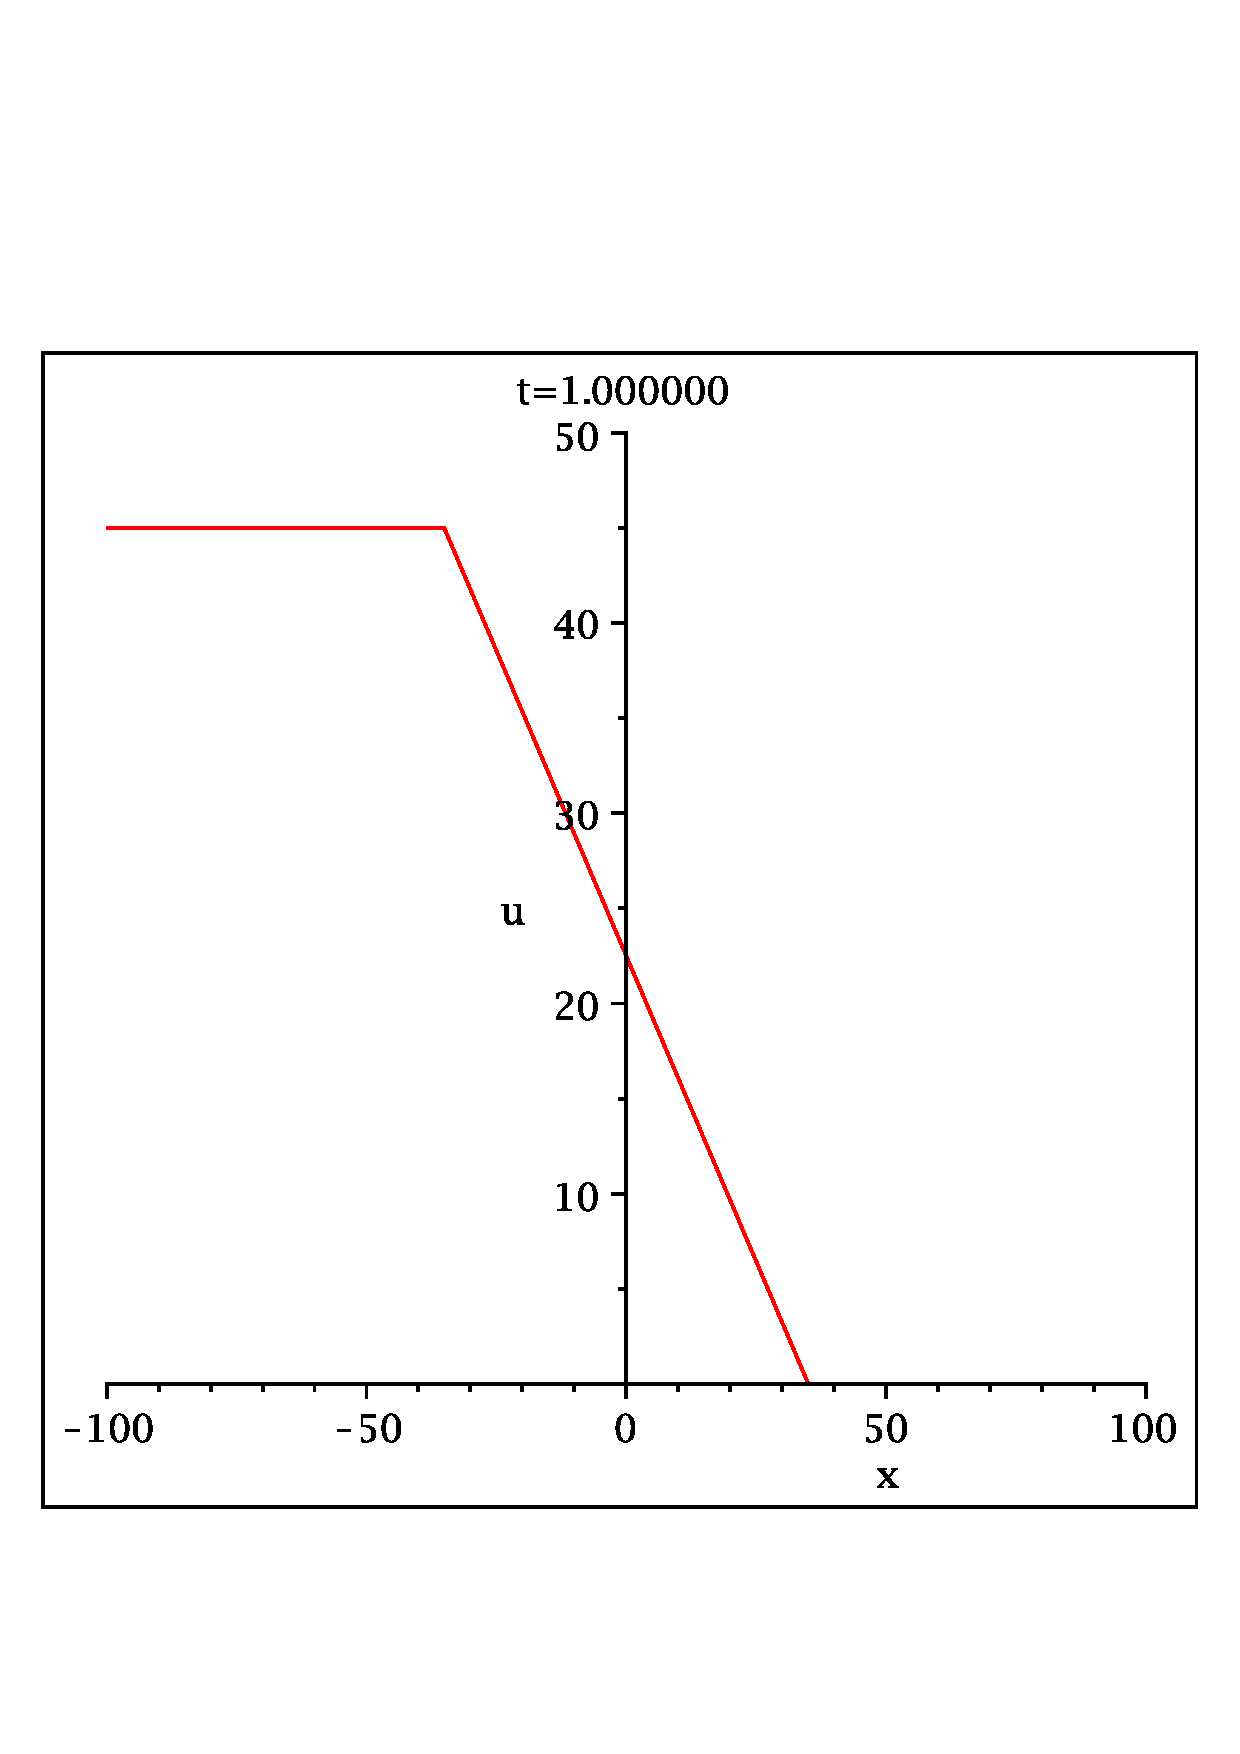
\includegraphics[width=55mm]{media/ex2-t2.pdf}} \quad 
                \subfigure{\includegraphics[width=55mm]{media/ex2-t3.pdf}}}
        \caption{Solution for exercise 2 plotted at time $t=0,1,2,3$}
        \label{fig:ex2-plots}
    \end{figure}

    \subsection*{c)}
    As can be seen in figure~\ref{fig:ex2-plots} the solution is a piecewise linear function. As time increases the point with $u=0$ moves further to right and the point with $u=\umax$ moves further to right. This corresponds to the cars that started from the red light moving further and further away from the traffic light towards right. The solution is therefore consistent with the physical intuition.

    \section*{Exercise 3}
    Continuing with the traffic flow PDE in (\ref{eq:pde-ex2}) we now model a queue building up at point $x=0$. To the left of $x=0$ there is a uniform density $u_0$ of cars. To the right of $x=0$ the density is $\umax$. Setting $u_0=\umax/2$ gives the initial condition
    \begin{equation*}
        u(x,0) = \phi_2(x) = \begin{cases}
            \frac{\umax}{2} & x < 0 \\
            \umax & x > 0
        \end{cases}
    \end{equation*}

    \subsection*{a)}
    Some of the characteristic curves in the $(x,t)$-plane should be drawn. For characteristic curves that crosses the $x$-axis on the negative side the ``slope'' is
    \begin{equation*}
        a(\phi_2(x)) = a(\umax/2) = 0
    \end{equation*}
    so these characteristic curves are vertical lines in the $(x,t)$-plane. For characteristic curves that crosses the $x$-axis on the positive side, the ``slope'' is
    \begin{equation*}
        a(\phi_2(x)) = a(\umax) = -\vmax
    \end{equation*}
    Using the previous two equations some of the characteristic curves are plotted and shown in figure~\ref{fig:characteristics-q3}.

    \begin{figure}[!ht]
        \centering
        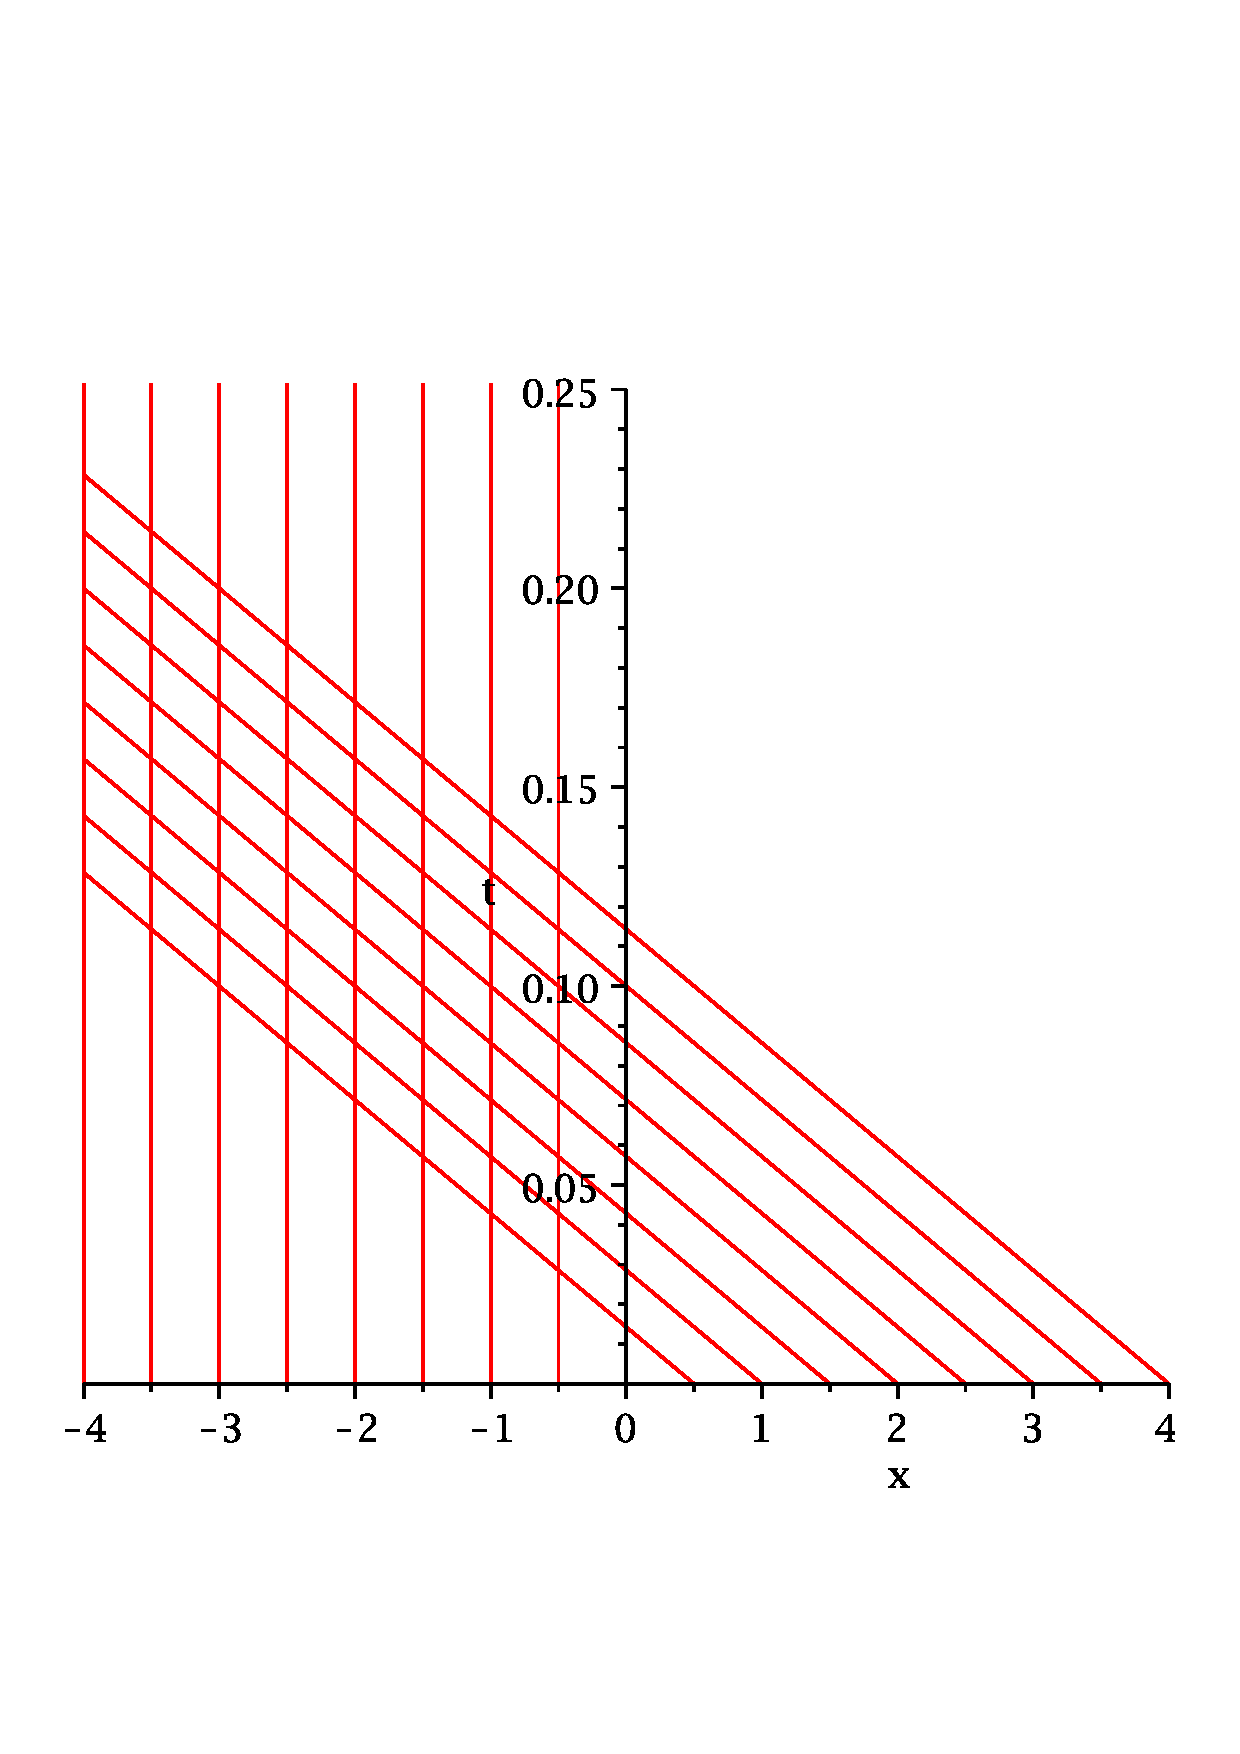
\includegraphics[width=60mm]{media/characteristics-ex3.pdf}
        \caption{Characteristic curves for exercise 3}
        \label{fig:characteristics-q3}
    \end{figure}

    From the figure it is seen that some of the characteristic lines crosses each other. Therefore a line in the $(x,t)$-plane exists where the solution $u$ will be discontinous.

    \subsection*{b)}
    The slope of the line of discontinuity is now found. The function $A$ is given by $A'(u) = a(u)$ so
    \begin{equation*}
        A(u) = \vmax\left(u-\frac{u^2}{\umax}\right)
    \end{equation*}
    Using equation 14.1.17 in the textbook the ``slope'' of the line of discontinuity can be found. First it is noticed that all characteristic curves, at the right side of the discontinous line, crosses the $x$-axis for $x>0$. Therefore $u^+=\umax$. Likewise we get that $u^-=\umax/2$. The slope is now found as
    \begin{align*}
        \frac{A(\umax) - A(\frac{\umax}{2})}{\umax - \frac{\umax}{2}} &= \frac{0 - \frac{\vmax\umax}{4}}{\frac{\umax}{2}} = -\frac{\vmax}{2}
    \end{align*}
    The line of discontinuity is now drawn, along with some of the characteristic curves, in figure~\ref{fig:characteristics-with-shock}.

    \begin{figure}[ht]
        \centering
        \includegraphics[width=70mm]{media/characteristics-ex3-with-shock.pdf}
        \caption{Characteristic curves for exercise 3 along with the line of discontinuity}
        \label{fig:characteristics-with-shock}
    \end{figure}

    \subsection*{c)}
    The solution to the PDE in (\ref{eq:pde-ex2}) with initial condition $u(x,0)=\phi_2(x)$ is now found. Using the characteristic curves from the previous section we can immediately write
    \begin{equation*}
        u(x,t) = \begin{cases}
            \frac{\umax}{2} & x < -\frac{\vmax}{2}t \\
            \umax & x > -\frac{\vmax}{2}t
        \end{cases}
    \end{equation*}
    where $u$ has a discontinuity along the line $x=-\frac{\vmax}{2}$. $u$ is therefore a weak solution to (\ref{eq:pde-ex2}).

    \subsection*{d)}
    As can be seen from the expression for $u$, the beginning of the queue moves further and further to the left as time increases.


\end{document}
